\documentclass[oneside,10pt,a4paper]{report}
\usepackage[a4paper, left=3cm, right=3cm, top=3cm, bottom=3cm, headsep=10mm, footskip=12mm]{geometry}
\usepackage[T1]{fontenc}
\usepackage[ngerman, english]{babel}    % mehrsprachiger Textsatz
% babel: letzte Sprache in Optionen zeigt die Sprache des Dokumentes
% und kann durch den Befehl \selectlanguage{} geaendert werden
% Passen Sie die Optionen des babel-Paketes nach Bedarf an!
\usepackage{float}
\usepackage{graphicx}
\usepackage{url}
\usepackage{pdflscape}
\usepackage{mathtools}
\usepackage{amssymb, amsmath, amstext}
\usepackage{amsthm}
\usepackage{xcolor}
\usepackage{nameref}
\usepackage{siunitx}
\usepackage{makecell}
\usepackage{hyperref}
\usepackage{enumitem}
\usepackage[superscript,biblabel]{cite}
\usepackage{caption}
\usepackage{subcaption}
\usepackage{tabularx} 			% Tabellen erzeugen
\usepackage{multirow}			 % Zeilen in Tabellenbearbeitung
\usepackage{multicol} 			% Spalten in Tabellenbearbeitung 
\usepackage{lmodern}                        % Ersatz fuer Computer Modern-Schriften 
\usepackage{amsmath}                                           % zum besseren Aussehen am Bildschirm
\usepackage{booktabs} % für schönere Tabellen
\usepackage{sidecap}
\usepackage{rotating} % für die Landscape-Umgebung
\usepackage{afterpage}
\definecolor{Bluetitle}{HTML}{1F3864}
\definecolor{softbluetitle}{HTML}{274D7E}
\definecolor{Greyish}{HTML}{5A5A5A}
%\renewcommand{\refname}{Reference}
\usepackage{array,multirow}
\newcommand{\specialcell}[2][c]{%
	\begin{tabular}[#1]{@{}c@{}}#2\end{tabular}}
\usepackage{titlesec}

\titleformat{\chapter}[display]
{\normalfont\bfseries}{}{0pt}{\Huge}

\usepackage{lipsum} 


\begin{document}
	
	\begin{titlepage}
		\begin{center}
			\begin{figure}[h!tbp]
				
\includegraphics[width=\linewidth]{HUlogo.PNG}
			\end{figure}
			\vspace*{2 cm}
			
			\textcolor{Bluetitle}{\textbf{\huge Parasitologie - Praktikum}}\par
			
			\vspace*{2cm}
			\textcolor{Greyish}{\textbf{Versuchsdurchführende}}\par
			\textcolor{Greyish}{Huyen Anh Nguyen (572309)}\par

			\vspace*{0.5cm}
			\textcolor{Greyish}{\textbf{Versuchsort}}\par
			\textcolor{Greyish}{Haus 14, Kursraum}\par
			\textcolor{Greyish}{Gruppe 4}\par

			
			\vspace*{2 cm}
			\textcolor{Greyish}{\textbf{Versuchsleiter}}\par
			\textcolor{Greyish}{Prof. Dr. Kai Matuschewski}\par
			\vspace*{0.5cm}
			\textcolor{Greyish}{\textbf{Versuchsbetreuer}}\par
			\textcolor{Greyish}{Dr. Alexander Maier (ANU)}\par
			\textcolor{Greyish}{Linnea Polito}\par
			\textcolor{Greyish}{Grit Meusel}\par
			\textcolor{Greyish}{Dr. Richard Lucius}\par
			\textcolor{Greyish}{Peer Martin}\par
			\textcolor{Greyish}{Manuel Rauch}\par
			\textcolor{Greyish}{Dr. Katja Müller}\par

			\vspace*{2 cm}
			\textcolor{Greyish}{Abgabe 15. August 2024}\par
			
			
			
		\end{center}
	\end{titlepage}

	
	\tableofcontents
	\chapter{Note from the Author}
	Das Protokoll ist eine Collection von Einzelprotokolle der Versuchen, die in den Parasitologiepraktikum durchgeführt wurde.\\
	Es wurden Methoden gezeigt, wie eine Spezies identifiziert, untersucht und dessen Verhalten analysiert werden kann.\\
	Aufgrund dieser Diversitäten an Versuchen, wird das Protokoll in drei Großkapiteln unterteilt. Ich fand es nach den Tierklassen zu unterteilen sinnvoll, auch wenn einige Versuche einen eigenen Kapitel verdient haben.
	
	
	\chapter{Hirudinea}	
	Hirudinea sind Egel die zu der Klasse Clitellata (Gürtelwürmer) gehören, wo auch die Regenwürmer dazuzählen. Die Arten die zu den Clitellata gehören, besitzen ein sogenanntes Clitellum (verdicktes mit Epidermis, Drüsengürtel), welches das Befruchtungsort für Eizelle und Spermazellen sind. Clitellaten sind Hermaphroditen. Um Selbstbefruchtung auszuschließen, befinden sich die Spermazellen in Spermatheken und die Gameten wandern erst bei der Kokonbildung zu den Clitellum.\\
	Unter den Hirudinea gibt es räuberische (Haemopis sanguisuga), parasitische (Hirudo verbana) und aasfressende Arten, die aquatisch, amphibisch oder auch terrestrisch leben können.
	Die räuberische Arten ernähren sich von Wirbellosen und die parasitische Arten von den Wirbellosen und Wirbeltieren, wobei letzteres nicht wirtsspezifisch sind. Sie befallen jedoch Wirbeltiere in der selben Klassen \cite{Kühkental}.
	Aufgrund der fehlenden Glidern bewegen sich die Hirudinea durch kriechend, schwimmend und raupenartig fort und nutzen dabei ihre Saugnapfen als Haftwerkzeug an Oberflächen.\\
	Mit mehr als 700 Arten unter den Hirudinea und mehr als 7400 Arten unter den Clitellaten ist es wichtig die Arten richtig zu bestimmen.  Dafür stehen mehrere Methoden zur Verfügung, dies zu tun. Eine davon ist die Dichotomische Bestimmungsmethode, welches Morphologisch das untersuchende Individuum systematisch zuordnet und die genetische Analyse mittels Polymerase Chain Reaction (abgekürzt: PCR).\\
	\\
	In den Kurs wird auch noch zusätzlich die Hirudinea mit den Oligochaeta (Wenigborster) verglichen.
	
	
	
		\section{Arten Bestimmung mittels dichotomischen Bestimmungs- schlüssel}\label{Abschnitt: DichoBestim}
			\subsection{Einleitung}
				Dichotomische Bestimmung ist eine Methode ein Individuum morphologisch und systematisch einer Reich, Stamm, Klasse, Ordnung und Gattung zuzuordnen und dessen Art zu bestimmen.\\
				Dichotomie kommt aus den altgriechisch und bedeutet grob übersetzt zweifacher Schnitt \cite{wiki_dichotom}.
				Der Dichotome Bestimmungsschlüssel ist eine Tabelle oder Liste von Merkmalen, die ein Experte augelistet hatte, womit das zu untersuchte Individuum abgeglichen werden kann. Dafür stehen zwei Merkmalen pro Kategorie zu (Es gibt auch Submerkmalen unter den Hauptmerkmalen, um auch kleine Abweichungen abzudecken), wo der Nutzer entscheidet welche Merkmale zu der Spezies zutrifft\cite{dichotomer_schlüssel}. Durch die Merkmalskomibantion kann somit das Taxa bestimmt werden.
			
			\subsection{Methode}
				Unter einem Stereomikroskop wurde ein in Ethanol fixiertes Egelprobe (Länge: 3 cm) untersucht.\\
				Die Merkmale wurden anhand des Dichotomischen Bestimmungsschlüssel der Egel Deutschlandsnach Clemens Großer auf Moodle systematisch zugeordnet.\\
				Damit die Probe nicht austrocknet, wurde in regelmäßigen Abstand die das Tier mit Wasser befeuchtet.
			
			\subsection{Ergebnis}
				In Figure \ref{fig:feuchte_augen} ist zu sehen, dass diese Spezies vier Augen in der vordere Reihe besitzt. Hinter der vorderen vier Augen gibt es pro Seite noch in diagonalen Stellung zwei Augen.\\
				\\
				Für die Artbestimmung wurde folgende Entscheidung getroffen:\\
				Augenzahl: 8 $\rightarrow$ 4 Augen in 1 vorderen Reihe, je 2 hinter liegenden, schräg gestellten Reihen $\rightarrow$  Dina, Erpobdella, Trocheta $\rightarrow$ der gesamter Körper abgeplattet; alle Ringe gleichbreit $\rightarrow$  Erpobdella $\rightarrow$  abgebrochen, aufgrund der knappen Zeit.\\
				\begin{figure}[H]
					\centering
					\begin{subfigure}[b]{0.55\textwidth}
						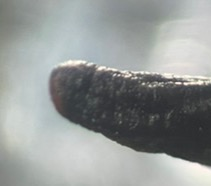
\includegraphics[width=\textwidth]{trockene_dichotom.jpg}
						\caption{Alte Egelprobe.}
						\label{fig: trockene_augen}
					\end{subfigure}
					\hfill
					\begin{subfigure}[b]{0.37\textwidth}
						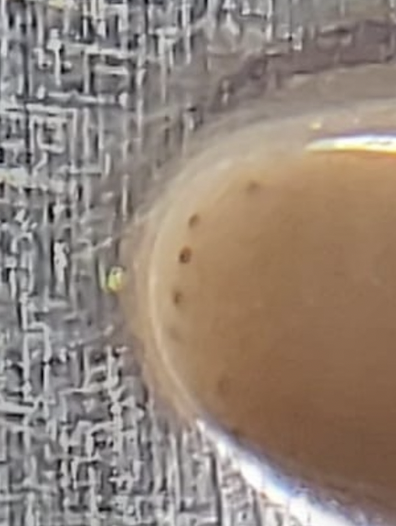
\includegraphics[width=\textwidth]{Dichotom_augen}
						\caption{Frische Egelprobe}
						\label{fig:feuchte_augen}
					\end{subfigure}
					\caption{Mikroskopische Aufnahme von den Vorderkopf der Egelproben. In Figure \ref{fig: trockene_augen} handelt sich um die Egelprobe, die hier für den Versuch untersucht wurde. Aufgrund des Zustandes der Probe wurde die die Augenlage von der Komiliton*in Melissas Probe (Figure \ref{fig:feuchte_augen}) untersucht. Beide Spezies gehören zur selben Art.}
					\label{fig: Dicho_augent}
				\end{figure}
			
			
			\subsection{Diskussion}
				Anhand des Dichotomischen Bestimmungsschlüssel wurde der vorliegende Egel zu der Gattung Erpobdella zugeordnet.
				Da der Versuch nachmittags durchgeführt wurde und die Exemplare schon vormittags verwendet wurde, war der Zustand des Egels nicht mehr optimal für eine ordentliche Bestimmung.
				Damit die richtige Art bestimmt werden kann, ist eine genetische Analyse von Vorteil. Die Verwendung des Dichotomischen Bestimmungsschlüssel muss geübt werden. Eine unerfahrende Person wird dabei oftmals eine falsche Entscheidung treffen, da viele Merkmale nicht so eindeutig sind wie in den Bestimmungsschlüssel beschrieben ist.\\
				Diese morphologische Methode kann aber mit einer DNA-Barcoding unterstützt werden, welches im nächsten Abschnitt behandelt wird.
		
		\section{Arten Bestimmung mittels DNA-Barcoding}
			\subsection{Einleitung}
				Die Art des Egels wird anhand seines Genoms bestimmt. 
				Dabei werden Markergens in der Spezies molekolar untersucht, die spezifisch für eine Art konserviert ist.\\
				Da jede Art einen einzigartigen genetischen Sequenzabfolge besitzt, eignet sich diese Methode bestens um eine Spezies zu phylogenetisch zu analysieren \cite{Folmer} \cite{Herbert}.\\
				Es setzt natürlich vorraus, dass die Sequenzabfolge irgendwo auf einer Datenbank zu der Art hinterlegt ist, um mit der zu untersuchende Spezies abzugleichen.\\
				Als Sequenzmarker wird die für das  Cytocrome C Oxidase subunit 1 Enzym (abgekürzt: COI) codierte Gen in den Mitochondrien verwendet. Mitochondrialer DNA besitzen keine Introns und wird haploid vererbt (COI wird maternal vererbt), so dass es nicht wie beim Kerngenom zwei verschiedene Varianten eines Gens existieren.\\
				Damit für die Sequenzierung genug DNA-Material zur Verfügung stehen, wird hier die Polymerase Chain Reaction (abgekürzt: PCR) verwendet.\\
				Das Verfahren ermöglicht eine schnelle und hohe Kopiezahl des gewünschten Genabschnittes zu bekommen.
				Für die PCR wird ein hitzestabiles DNA-Polymerase I-Enzym (Taq-Polymerase aus dem Thermus aquaticus-Bekterium) benötigt, da die Doppelsträngige DNA zu Einzelsträngige DNA denaturiert werden muss.
				Damit die Taq-Polymerase die Amplifikation (Vervielfältigung der Nukleinsäure) durchführen kann, beötigt diese neben den Nukleotiden auch Primer, die an beide DNA-Stränge (Codogener Strang und nicht codogener Strang) an den gewünschten Genbereich bindet. Hier wird der Forward-Primer LCO1490 und Reverse Primer HC02198 von Folmer (1994) verwendet (siehe Table \ref{tab: Primer}), welches ermöglicht im GOI-Gen ein 659 bp langes Genfragmentes zu amplifizieren.\\
				Im Anschluss wird mittels einer Agarosegelelektrophorese die Fragmente nach der Größe aufgetrennt und sequenziert.\\
				
			
			\subsection{Methode}
				\textit{14. Juni 2024}\\
				\\
				Für die gDNA-Isolierung wurde das Genomic DNA tissue kit verwendet.\\
				Ein grobes Stück Egelgewebe (grob 20 mg) wurde mit einem Skalpell homogenisiert und mit 400 $\mu$L Lysispuffer und 25 $\mu$L Proteinase K für 30 Minuten bei 56°C unter Schütteln inkubiert. Dann wurden 250 $\mu$L Bindingsolution SBS zugegeben und gemischt und auf einer Zentrifugenröhrchen überführt. Diese wurde für 2 Minuten bei 10000 x g zentrifugiert und das Filtrat verworfen.\\
				Dann wurde 600 $\mu$L Waschpuffer auf die Säule pipettiert und für 1 Minute für 11000 x g zentrifugiert und dieser Schritt wurde mit 300 $\mu$L Waschpuffer wiederholt. Am Ende des wurde auf maximalen Speed für 30 Sekunden die Überreste an Lösungsmittel abzentrifugiert.\\
				Das Zentrifugenröhrchen wurde auf einem 1.5 mL Eppendorf-Röhrchen überführt und auf dem Filter 50 $\mu$L RNase freies Wasser pipettiert und mit geöffneten Deckel bei 11000 x g für 2 Minuten zentrifugiert.
				\\
				\textit{12. Juli 2024}\\
				\\
				Die Konzentration vom gDNA wurde photometrische bestimmt und beträgt 15.2 mg/mL (Wurde von Grit Meusel durchgeführt).
				Es wurden 2 $\mu$L gDNA und als negativ Kontrolle 2 $\mu$L Wasser mit 23 $\mu$L Mastermix (Pipettierschema für den Mastermix siehe Table \ref{tab: Mastermix-Pipettierschema}).
				Die Proben werden dann für 34 Cyclen amplifiziert (PCR-Cyclen siehe Table \ref{tab: PCR-Cyclen}).
				\\
				\textit{14. Juni 2024}\\
				\\
				5 $\mu$L amplfizierte PCR-Proben wird mit 1 $\mu$L 6x Gel-Puffer vermischt und auf einem 1$\%$igen Agarosegel aufgetragen. Zusätzlich wird ein DNA Marker mitraufpipettiert für die Größenbestimmung.
				Der Gellauf lief bei 100V für 1 Stunde und wurde unter ultravioletes Licht analysiert. Die Sequencebestimmung wird von den Versuchsbetreuer durchgeführt.\\
				\\
				Die Sequenzabfolge wird mit der National Library of Medicine-Datenbank abgeglichen und ein Alignment-Tree in MegaX erstellt.
				
			
			\subsection{Ergebnis}
				In Figure \ref{fig:Agarosegel} ist zu erkennen, dass es bei der Probe eine Bande existiert. Die Amplifikation hat DNA-Fragmente produziert, die bei circa 600 bp liegt. Die Negativ Kontrolle zeigt keine Bande.
				
				\begin{figure}[H]
					\centering
					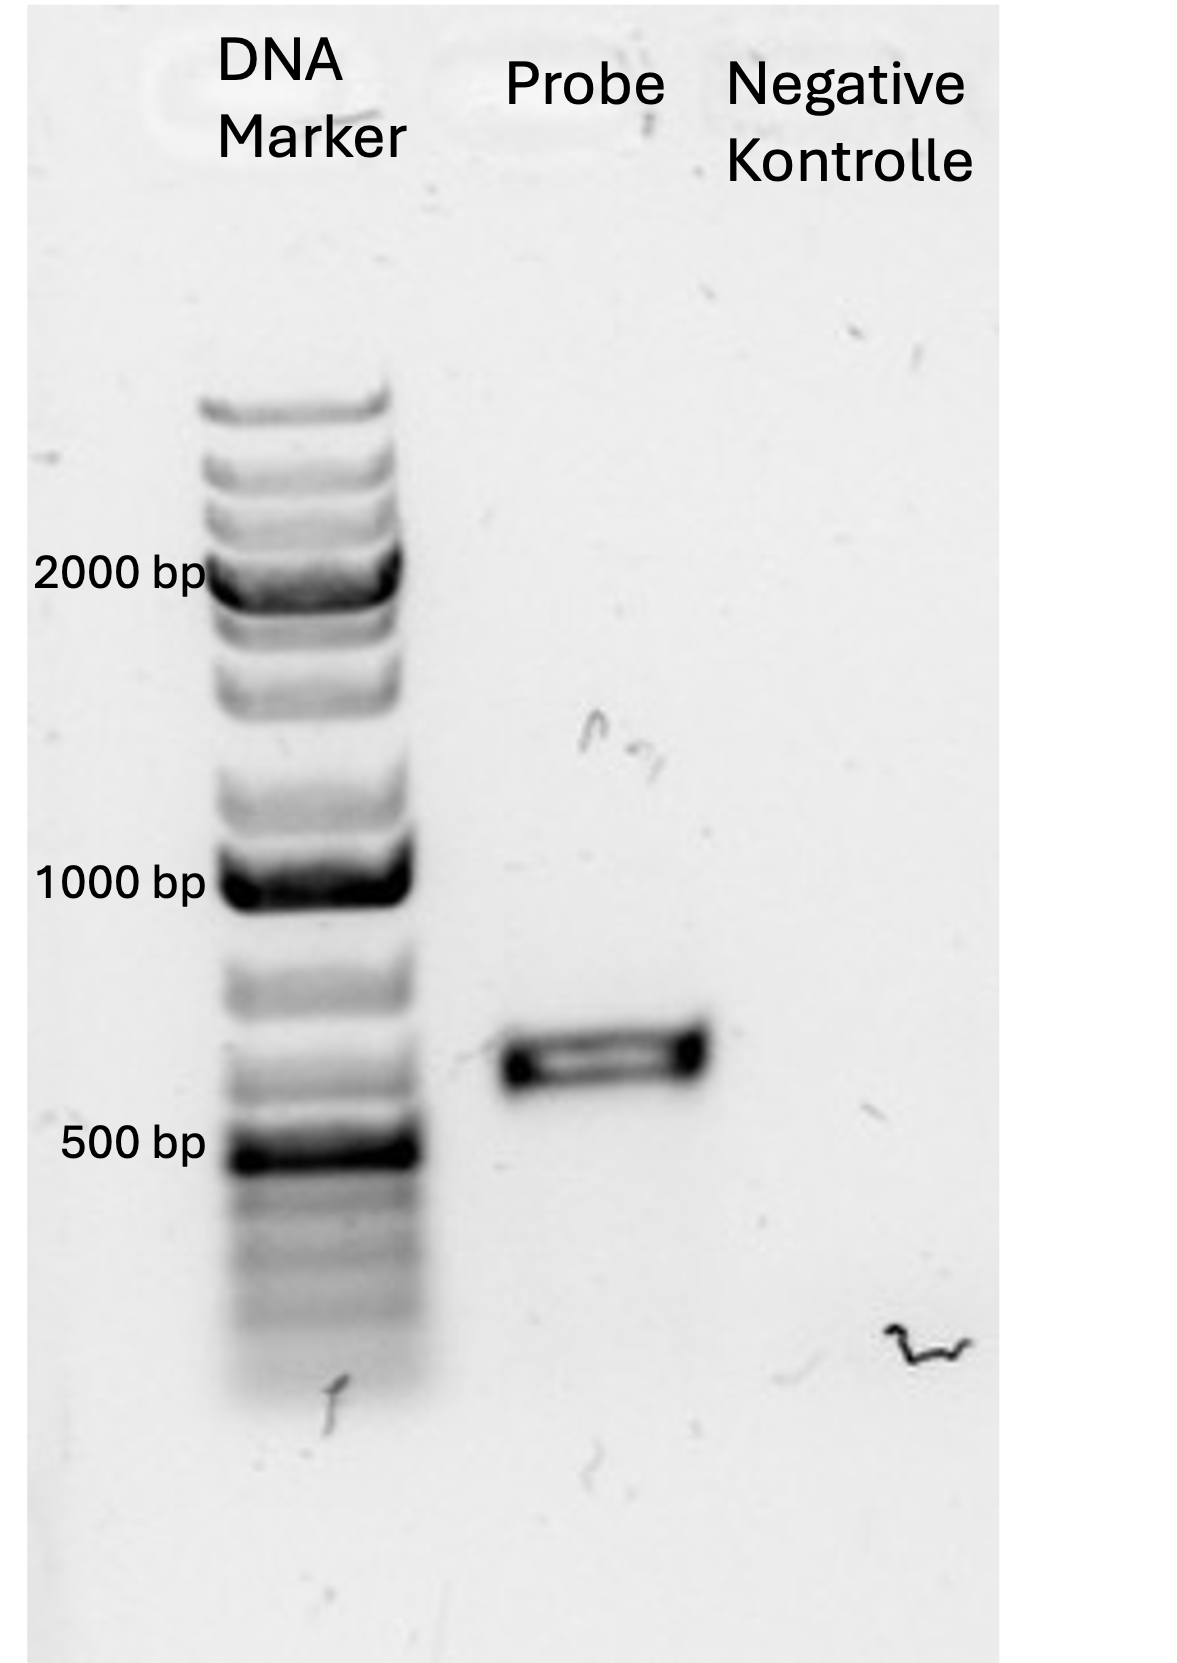
\includegraphics[scale=0.7]{gel.png}
					\caption{Größenauftrennung der gDNA PCR-Probe von der unbekannte Egelgewebestücks und der Negativkontrolle (Wasser) aufgetrennt auf einer 1$\%$-Agarosegel mit einem DNA-Marker als Größenvergleich.}
					\label{fig:Agarosegel}
				\end{figure}
				
				Die Sequenz von der Isolierte Bande aus Figure \ref{fig:Agarosegel} ist in Table \ref{tab: Consensus-Sequenz Gruppen 1-7} dargestellt und glich mit 99.49 $\%$ mit der Art Erpobdella octoculata zusammen. Die Referenzsequenz stimmt mit der Art Erpobdella testacea mit der Datenbank zu 99.69 $\%$ überein.\\
				Bei der MUSCLE Alignment Algorithmus zeigen das beide Sequenzen 266 gemeinsame Basenpaare besitzen. \\
				In Figure \ref{fig: Baum} wurden die beiden Arten mit 9 weiteren Arten in Relation aufgestellt und mit der Maximum Parsimony Algorithmus den Verwandschaftsgrad bestimmt.
				
				\begin{figure}[H]
					\centering
					\includegraphics[scale=0.7]{Anhs Tree.png}
					\caption{Aligmenttree mit 10 Arten. Es wurde nach dem MUSCLE-Algorithmus alignt und ein Baum nach dem Maximium Parsimony Methode erstellt. Die Spezies die in den Kurs untersucht wurde trifft mit 99.49 $\%$ dem Erpobdella octoculata zu. Die Verwandschaftsbeziehung zu Erpobdella testacea, welches die Referenzsequenz vom Betreuer zur Verfügung stand ist in diesen Figure dargestellt. Die Rohsequenzen von der DNA-Sequenzierung ist in Table \ref{tab: Consensus-Sequenz Gruppen 1-7}}
					\label{fig: Baum}
				\end{figure}
				
			
			\subsection{Diskussion}
				Es wurde ein Sequenz amplifiziert, dass 664 bp lang ist (siehe Table \ref{tab: Consensus-Sequenz Gruppen 1-7}), welches in der Agarosegelelektrophorese auch in den Bandenbereich von circa 600 bp aufgetrennt wurde.\\
				Der Sequenzvergleich mit der Datenbank der National Library of Medicine wurde der im Versuch zu untersuchten Egel der Art Eropbdella octoculata mit einer Übereinstimmung von 99.49 $\%$.  
				In Abschnitt \ref{Abschnitt: DichoBestim} wurde anhand des Dichotomischen Bestimmungsschlüssel morphologisch die Gattung Erpobdella von den Egel bestimmt und mit der DNA-Barcoding wurde diese Gattung bestätigt.
				Der bestimmte Egelart Eropbdella octuculata und Erpobdella testacea bilden keine monophyletische Gruppe, wenn andere Egelarten in Bezug genommen wird (siehe Figure \ref{fig: Baum}) und mittels MUSCLE Alignment- und Maximum Parsimony-Algorithmus analysiert wird.\\
				Die Artenbestimmung mit der DNA-Barcoding ist deutlich kostspieliger und zeitaufwendiger als die Methode mit dem dichiotomischen Bestimmungsschlüssel. Mit beiden Methoden konnte die gleiche Gattung bestimmt werden.
				Die Sicherheit des Ergebnis ist bei beiden Methoden Abhängig von den gesammelten Daten beziehung der vorliegende Daten.\\
				
		\section{Vergleich Hirudinea und Regenwurm}
			\subsection{Einleitung}
				In der Gruppe der Clitellata gehören die Oligochaeta (Wenigborster) und die Hirudinea (Egel), die zu der großen Gruppen der Anneliden (Ringelwürmer) gehören.
				Die Oligochaeta ist ein Sammelbegriff für Paraphyletische Gruppe die hier keine Monophyletische Gruppe bilden. Aus den Oligochaeta wird hier der Regenwurm Lumbrius terrestris als Vertreter auserwählt. Der Regenwurm ist der bekannteste REgenwurmart in Europa und lebt in den Boden von Wiesen und Gärten \cite{regenwurm}. Sie gehören zu den Destruenten und sind für das Ökosystem ein wichtiger Bestandteil. Von den Hirudinea wird der medizinischer Egel Hirudo verbana als Vertreter genommen. Der Egel ist ein Ektoparasit, welches sich von Fischen, Amphibien und Wirbeltieren ernährt  und in den Gewässern der Mittelmeerraum vorkommt \cite{hirudo}. Sie haben in der Medzinin (weswegen auch dieser Umgangsname) eine besondere Bedeutung, da ihr Speichel gerinnungshemmend, blutsenken, entzündungshemmend und lokal betäubend wirkt.\\
				In diesen Versuch werden von den beiden Arten die Körpersysteme morphologisch auf Unterschiede und Gemeinsamkeiten untersucht.\\
				
				
			\subsection{Methode}
				Der Hirudo verbana - Egel wurde unter einem Stereo-Mikroskop präperiert und auf einem mit Alufoliebedeckten Styroformplatte fixiert. Entlang der Mittelline der Bauchseite wurde die Bauchseite mit der stumpfen Seite der Schere aufgeschnitten und aufgefächert fixiert. Der Verdauungstrakt wurde betrachtet und vorsichtig abgenommen um den inneren Rückenbereich mit den Geschlechtsorganen und Harnsystem zu betrachten. Das Nervensystem konnte nicht erkannt werden.\\
				Die Morphologie wurde dann mit den Regenwurm aus MB5 (Lumbricus terrestris) verglichen.
			\subsection{Ergebnis}
				
				In Table \ref{tab: Egel vs Regenwurm} sind die Merkmale von den Hirudo verbana und Lumbricus terrestris für die Organsysteme Verdauungs-, Kreislauf-, Nerven-, Harnsystem und Fortpflanzungsorgane aufgelistet. 
				\begin{table}[H]
					\centering
					\caption{Merkmale in den Organsysteme zwischen der Hirudo verbana (Egel) und Lumbricus terrestris (Regenwurm). Die Merkmale sind in Figure \ref{fig:Egel_ana} (Hirudo verbana) und \ref{fig:Regenwurm_ana} (Lumbricus terrestris) zu sehen.}
					\label{tab: Egel vs Regenwurm}
					\begin{tabular}{c c c}
						\toprule
						& Hirudo verbana & Limbricus terrestris\\
						\midrule
						\multirow{7}{*}{\parbox[t]{2cm}{Verdauungs- system}} & \multirow{7}{*}{\parbox[t]{6cm}{Der Magen erstreckt sich über die Körperlänge und der Egel besitzt einen an den Magen 10 Zweipaarige Blindsäcke, wo das letzte Paar vergrößert ist. Am Vorderernde befindet sich Kifern mit Zähnen aus Kalzit und daran der Pharynx}}&\multirow{7}{*}{\parbox[t]{6cm}{Der Mund geht zu den Pharynx über diese zu den Oesophagus mit den Kalksäckchen. Bevor es zu den Muskelmagen übergeht, ist da noch der Kropf. Der Magen ist nur zwei Segmente lang und geht dann zu den Darmtraktes über.}}\\
						&&\\
						&&\\
						&&\\
						&&\\
						&&\\
						&&\\
						\midrule
						\multirow{5}{*}{\parbox[t]{2cm}{Kreislauf- system}}& \multirow{5}{*}{\parbox[t]{6cm}{Lateralkanäle und Seitenkanäle durchziehen den Egel und in der Mitte des Körpers das Dorsalgefäß}}&\multirow{5}{*}{\parbox[t]{6cm}{Das Rückengefäß ist auf dem Darm und besitzt Gefäßschlingen die das Blut zu den Bauchgefäß pumpt. Die Gefäßschlingen wird auch Lateralherz genannt}}\\	
						& &\\
						&&\\
						&&\\
						&&\\
						\midrule
						\multirow{2}{*}{\parbox[t]{2cm}{Nervensystem}} & \multirow{2}{*}{\parbox[t]{6cm}{Besitzt ein Cerebralganglion unterhalb des Kiefers}}&\multirow{2}{*}{\parbox[t]{6cm}{Am Vorderen Ende befinden sich zwei Cerebralganglien}}\\
						& &\\
						\midrule
						\multirow{4}{*}{\parbox[t]{2cm}{Fort- pflanzungs- organe}} & \multirow{4}{*}{\parbox[t]{6cm}{Räumlich getrennte Geschlechtsorgane. Besitzt Vagina und eine Penistasche. Über den ganzen Körper sind die Hoden verteilt.}}&\multirow{4}{*}{\parbox[t]{6cm}{Weiblicher und Männliche Geschlechtsorgane sind räumlich voneinander getrennt. Besitzt keine Vagina oder Penis.}}\\
						& &\\
						&&\\
						&&\\
						\midrule
						\multirow{3}{*}{\parbox[t]{2cm}{Harnsystem}}& \multirow{3}{*}{\parbox[t]{6cm}{Besitzen lateral paarige  Harnblasen mit Nephridien die über das ganze Körper verteilt sind}}&\multirow{3}{*}{\parbox[t]{6cm}{Besitzen paarige Nephridienschlingen in jeden Segmenten, die lateral liegen}}\\
						& &\\
						&&\\
						\bottomrule
					\end{tabular}
				\end{table}
				
			\subsection{Diskussion}
				Hirudo verbana und Lumbricus terrestris zeigen viele gemeinsame Merkmale wie die kräftigen Ring und Längsmuskulatur unter der Haut und wiederholende Organe pro Segmente wie die Nephridien und Blutgefäße. Beide Besitzen weibliche und männliche Geschlechtsorgane, die räumlich durch Segmente getrennt sind, um Selbstbefruchtungen zu verhindern.\\
				Durch die verschiedene Ernährungsweisen, ist bei den Verdauungssystem die größsten Unterschiede zu sehen. So hat der Egel aufgrund seines Lebensform einen stark vergrößerten Magen, da diese Art für eine sehr lange Periode ohne Nahrung überleben kann und wenn es ein Wirt findet, sich vollsaugt, bis auch die Blindsäcke voll sind. Wenn diese vollgesaugt ist, pflanzen sich die Tiere sich fort. Zudem hat der Egel Kiefer mit Zähne um sich an den Wirt haften zu können und ins Fleisch reinbeißen zu können. Der Regenwurm hingegen ernährt sich von toten Pflanzenreste und benötigt ein starken muskulösen Magen, um zusammen mit den eingesaugten Sand diese zerkleinern zu können. Zudem hat der Regenwurm noch zusätzlich einen Kalksäckchen, dessen funktion noch nicht ganz klar ist \cite{Kühkental}. 
				
	
	
	\chapter{Trematoden}
		Trematoden (Saugwürmer) gehören zu der Klasse der Plathelminthes (Plattwürmer) und bilden mit den Cestoda eine monophyletische Gruppe.\\
		Die meisten Trematoden sind Endoparasitisch und nutzen Wirbellosen als Zwischenwirt und Wirbeltieren als Endwirt.\\
		Die Entwicklungszyklen der Trematoden ist abhängig vom Wirts- und Generationswechsel. Bei der Generationswechsel wird von der sexuellen zu der asexuellen Phase gewechselt.
		Sie besitzen am Mund und Bauch Saugapparate, mit denen sie sich an dem Wirt haften können. Bis auf die Schistosoma sind die Trematoden zwittrig.
		\section{Einleitung}
			Dicrocoelium dendriticum nutzen als Zwischenwirt gerne Wirbellose Tiere wie die Schnecke und auch Ameisen.
			
		\section{Methode}
			\subsection{Malzacherfärbung}
			Die in 70$\%$ Ethanol fixierten adulten Dicrocoelium dendriticum wurden für 5 Minuten in Boraxcarmin fixiert und danach für 1 Minute lang in Leitungswasser differenziert bis das Gewebe zu rosa verblasste.\\
			Dann wurde für 5 Minuten in Strablaulösung (1$\%$ Astrablau, 3$\%$ Weinsäure in ddH$_2$O) gefärbt und anschließend für 2 Minuten in 3$\%$ Weinsäure solange entfärbt, bis das Gewebe rosa-lila wurde.
			Dann wurde das Objekt für 10 Minuten in 50$\%$ Ethanol, zwei Mal 10 Minuten 70$\%$, 10 Minuten in absoluten Ethanol und dann 5 Minuten zwischen zwei Objekträgern in absoluten Ethanol entwässert. Als letzter Entwässerungsschrit wurde das Objekt für 5 Minuten in absoluten Ethanol gelegt.\\
			Vor dem Eindecken wurde das Objekt für 10 Mintuen in Wintergrünöl inkubiert.\\
			
			
			\subsection{Trematodenlarvenisolation aus einer Wasserschneckenleber}
				Mit einer Pinzette wird ein Stück mit Trematoden infiziertes Wasserschneckenleber in Wasser zerrupft. Ein Tropfen des zerrupften Lebergewebe wird unterm Mikroskop nach den Larven untersucht.
		\section{Ergebnis}
			\subsection{Portrait des adultes Dicrocoelium dendriticum}
				\begin{figure}[H]
					\centering
					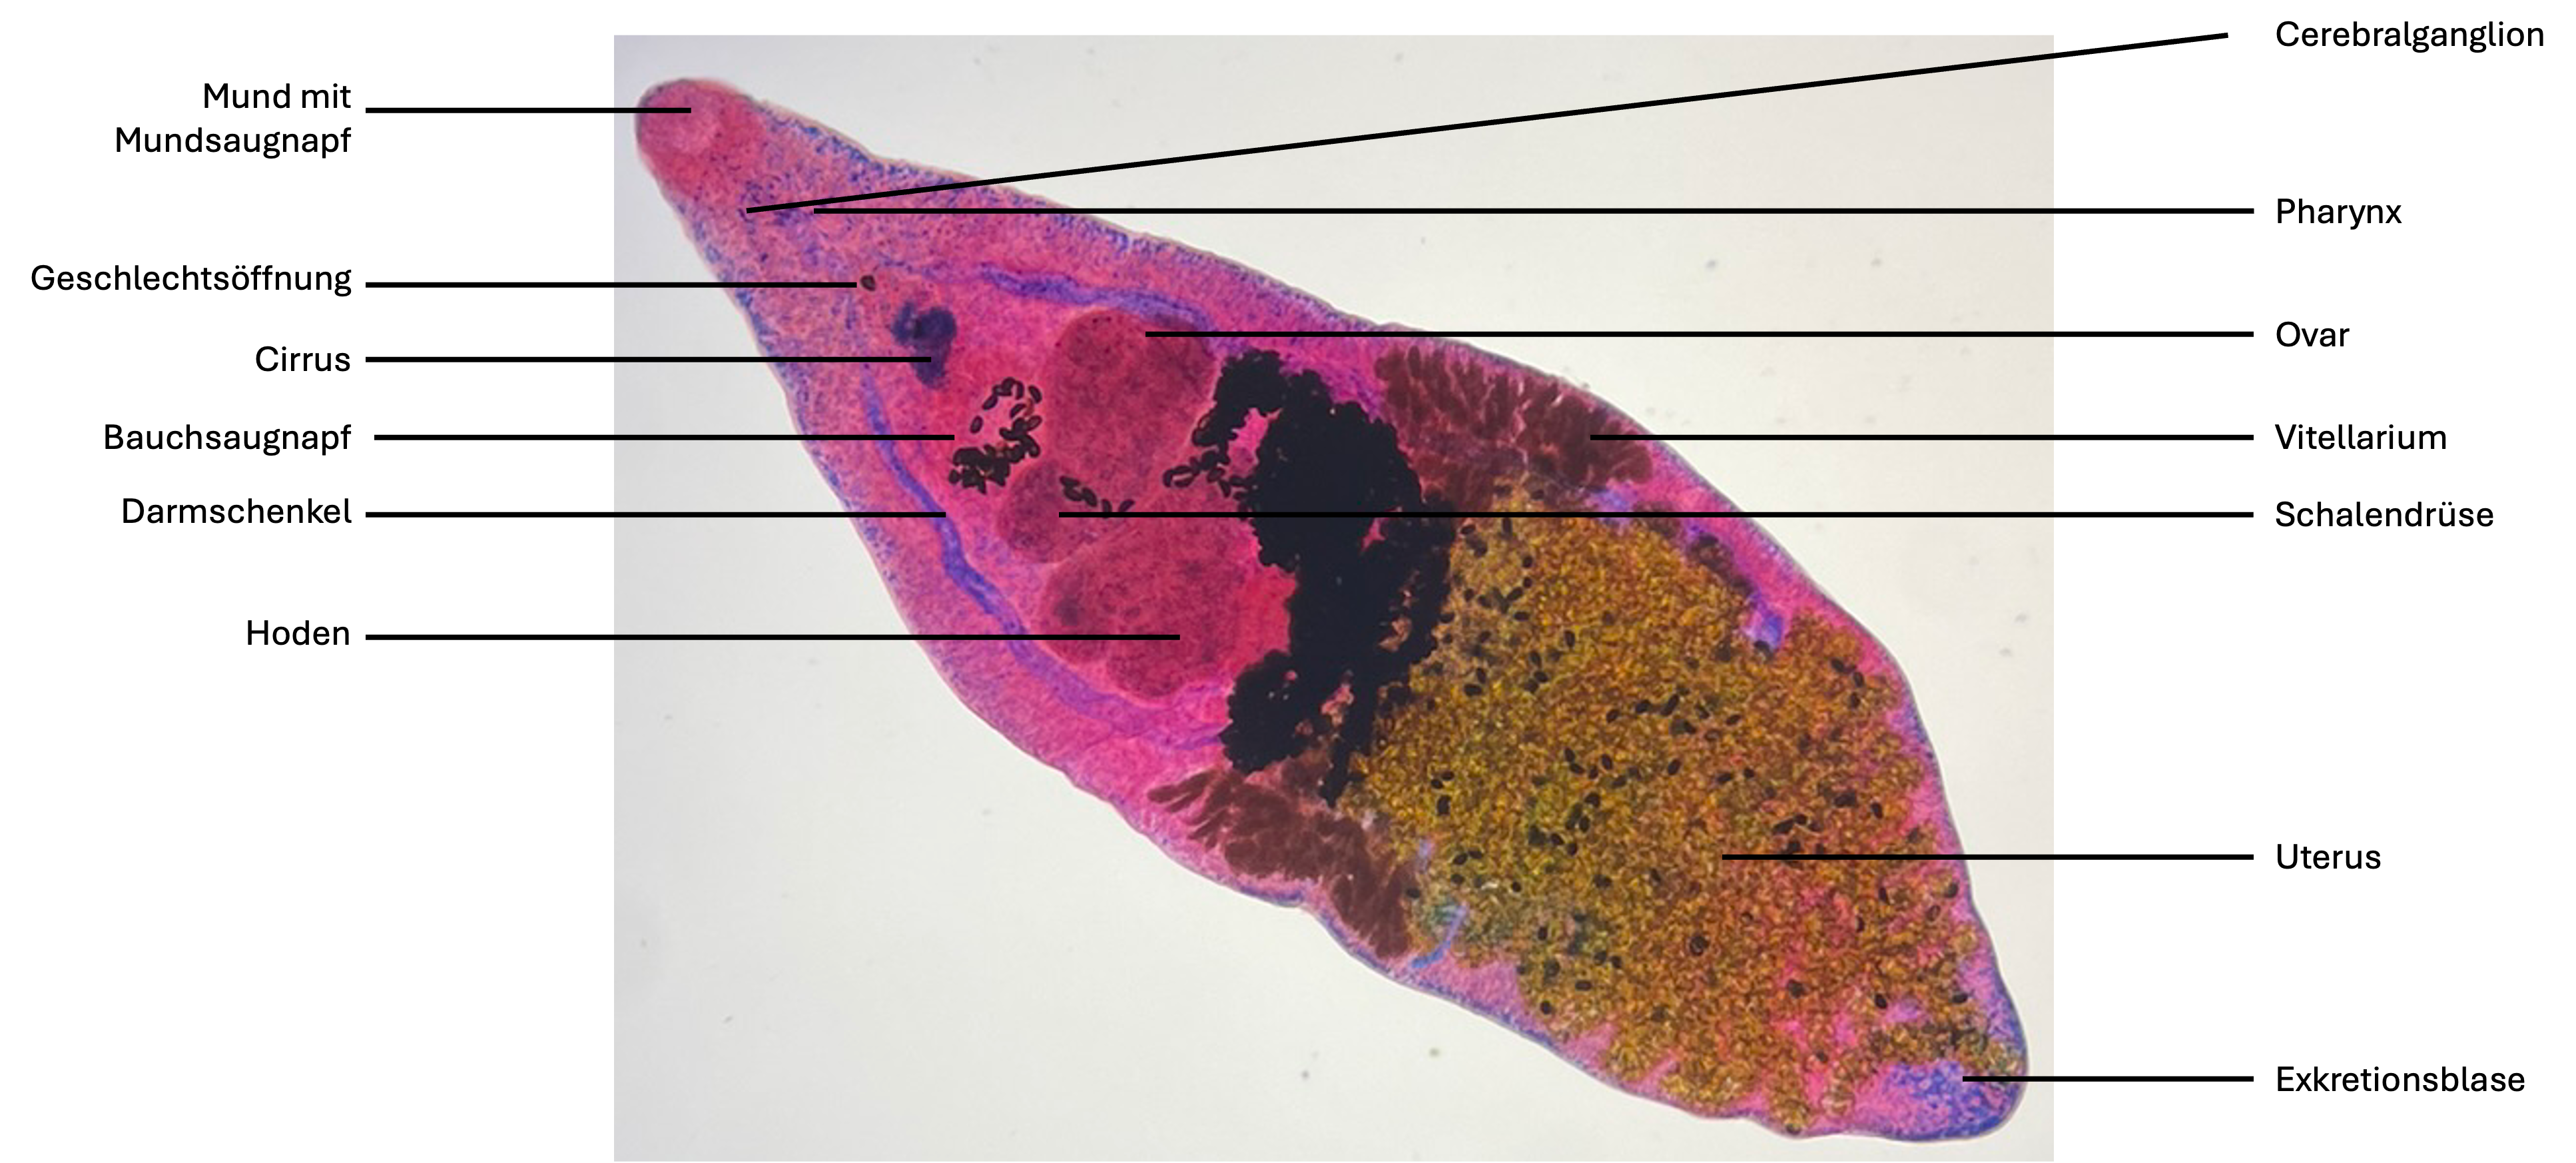
\includegraphics[scale=0.75, angle = 90]{Dicrocoelium dendriticum.png}
					\caption{40-fache Vergrößerung einer Malzacher-Färbung des adultes Dicrocoelium dendriticum (Leberegel) aus einer infizierten Wasserschneckenleber.}
					\label{fig: TrematodenMalzacherfärbung}
				\end{figure}
			\subsection{Trematodenlarven}
				In der Leberprobe wurden nur Larven in der Redie-Stadium gefunden (Figure \ref{fig: Trematodenlarven}).\\
				Es wird vermutet, dass die Schnecke viel zu früh gestorben ist, so dass aus den Redie-Stadium keine weiteren Entwicklungsstadien ermöglich werden kann.
				\begin{figure}[H]
					\centering
					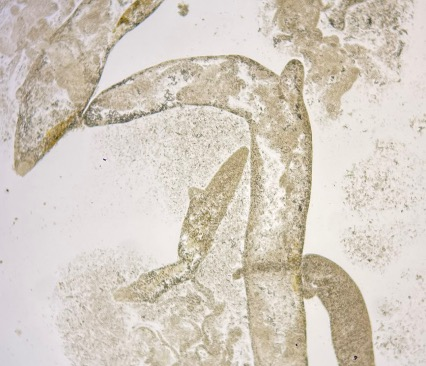
\includegraphics[scale=0.5]{Trematodenlarven.jpg}
					\caption{40-Fache Vergrößerung des Larvenstadium: Redie.}
					\label{fig: Trematodenlarven}
				\end{figure}
				
		
	
	\chapter{Plasmodium}
		\section{Giemsa-Färbung von infizierten Humanblutes}
			\subsection{Einleitung}
			\subsection{Methode}
			\subsection{Ergebnis}
			\subsection{Diskussion}
	
		\section{Darminhaltes des Blaberus craniifer}
			\subsection{Einleitung}
			\subsection{Methode}
			\subsection{Ergebnis}
			\subsection{Diskussion}
		
		\section{Cytochalasin D Wirkung auf die Motilität von Gregarinen}
			\subsection{Einleitung}
			\subsection{Methode}
			\subsection{Ergebnis}
			\subsection{Diskussion}
			
	
	
	\chapter{Anhang}
		\section{PCR}
		\begin{table}[H]
			\centering
			\caption{MasterMix Pipettierschema für 3 PCR-Raktionen. Der MasterMix ist 3-Fach konzentriert}
			\label{tab: Mastermix-Pipettierschema}
			\begin{tabular}{cc}
				\toprule
				& Volumen in $\mu$L\\
				\midrule
				10x Reaktionspuffer & 7.5 \\
				Oligo for & 1.5\\
				Oligo rev & 1.5\\
				dNTP Mix & 1.5\\
				Taq Polymerase & 0.3\\
				H$_2$O & 57\\
				\bottomrule
			\end{tabular}
		\end{table}
		
		
		\begin{table}[H]
			\centering
			\caption{PCR-Cyclus Einstellungsprogramm. 34 Cyclen wurde durchgeführt.}
			\label{tab: PCR-Cyclen}
			\begin{tabular}{cc}
				\toprule
				94°C & 3 Minute\\
				94°C & 45 Sekunde\\
				48°C & 45 Sekunde\\
				72°C & 1 Minute\\
				72°C & 5 Minute\\
				4°C & unendlich\\
				\bottomrule
			\end{tabular}
		\end{table}
		
		\begin{table}[H]
			\centering
			\caption{Sequenz vom Forward- und Reverse-Primer für die PCR. Folmer (1994).}
			\label{tab: Primer}
			\begin{tabular}{cc}
				Forward & 5’ GGTCAACAAATCATAAAGATATTGG 3'\\
				Reverse & 5’ TAAACTTCAGGGTGACCAAAAAATCA 3’\\				
			\end{tabular}
		\end{table}
		
		\begin{table}[H]
			\centering
			\caption{Consensus-Sequenz Gruppen 1-7. Die Bande im Bereich 600 bp wurde aus der Agarosegelelektrophorese isoliert und sequenziert.}
			\label{tab: Consensus-Sequenz Gruppen 1-7}
			\begin{tabular}{l}
				TTTATTCTAGGAAGCATGGGTCAGCTATAGCTGGCACAGGCATAAGGGTACTAATTCGAA\\
				TTGAGTTAGCCCAACCTGGCACATTTTTAGGAAACGATCAAATTTATAACACTATTGTAA\\
				CCGCTCACGGGCTAGTAATAATTTTCTTTATAGTAATACCTATTTTAATTGGAGGATTTG\\
				GAAATTGGTTGATTCCATTAATAATTGGTGCACCAGATATAGCCTTTCCTCGACTCAATA\\
				ATCTAAGATTTTGACTATTACCCCCATCAATAATTATATTAGTCTTCTCTGCATTTGTAG\\
				AAAATGGTGTGGGTACTGGATGAACAGTATACCCTCCCTTAGCATATAATATTGCCCACT\\
				CTGGCCCATCAGTAGATATGGCTATTTTCTCATTACATTTAGCAGGAGCTTCATCTATTT\\
				TAGGATCATTAAACTTTATTTCCACTGTAGCAAATATACGATGAAAAGGTATATCATTAG\\
				ATCGAATCCCTTTATTTATTTGATCAGTAATTATTACTACAGTACTTCTACTTCTATCAT\\
				TACCAGTTTTAGCAGCTGCCATTACTATATTACTGACTGATCGAAACTTAAATACATCCT\\
				TCTTTGACCCTGCAGGAGGAGGAGACCCAATCCTATTCCAACATTTATTTTGATTTTTTG\\
				GTCACC\\
			\end{tabular}
		\end{table}
		
		\begin{table}[H]
			\centering
			\caption{Consencus-Referenzsequenz vom anderen morphologischen Tier vom Betreuer zur Verfügung gestellt.}
			\label{tab: Vergleichssequenz}
			\begin{tabular}{l}
				TTTTAGGGGCCTGATCAGCTATAGCTGGTACAGGCATAAGAGTACTAATTCGAATTGAAT\\
				TAGCTCAACCCGGCACATTTCTAGGAAATGATCAAATTTATAATACTATTGTAACCGCAC\\
				ATGGATTAGTAATAATCTTCTTTATAGTAATACCTATTTTAATTGGAGGATTTGGTAATT\\
				GGTTAATTCCATTAATAATTGGGGCCCCAGATATAGCATTTCCGCGACTTAATAATCTAA\\
				GATTCTGACTACTTCCACCATCCATAATTATACTAGTATTCTCTGCATTTGTAGAAAATG\\
				GAGTAGGTACTGGATGAACAGTATACCCTCCTCTAGCATACAATATTGCACACTCTGGCC\\
				CATCTGTAGATATAGCTATCTTCTCATTACATTTAGCGGGAGCATCATCTATCCTAGGGT\\
				CCCTAAATTTTATTTCAACTGTAGCTAATATACGATGAAAAGGAATAACTATAGATCGAA\\
				TTCCTTTATTTATTTGATCAGTAATTATTACTACAGTTCTTTTACTACTCTCCTTACCTG\\
				TACTAGCAGCAGCAATTACAATATTATTAACTGATCGAAACCTAAATACATCATTCTTTG\\
				ACCCAGCAGGTGGAGGAGATCCTATTTTATTCCAACACTTATTTTGATTTTTTG\\
			\end{tabular}
		\end{table}
		
		\section{Anatomische Zeichnung Regenwurm und Medizinischer Egel}
		\begin{figure}[H]
			\centering
			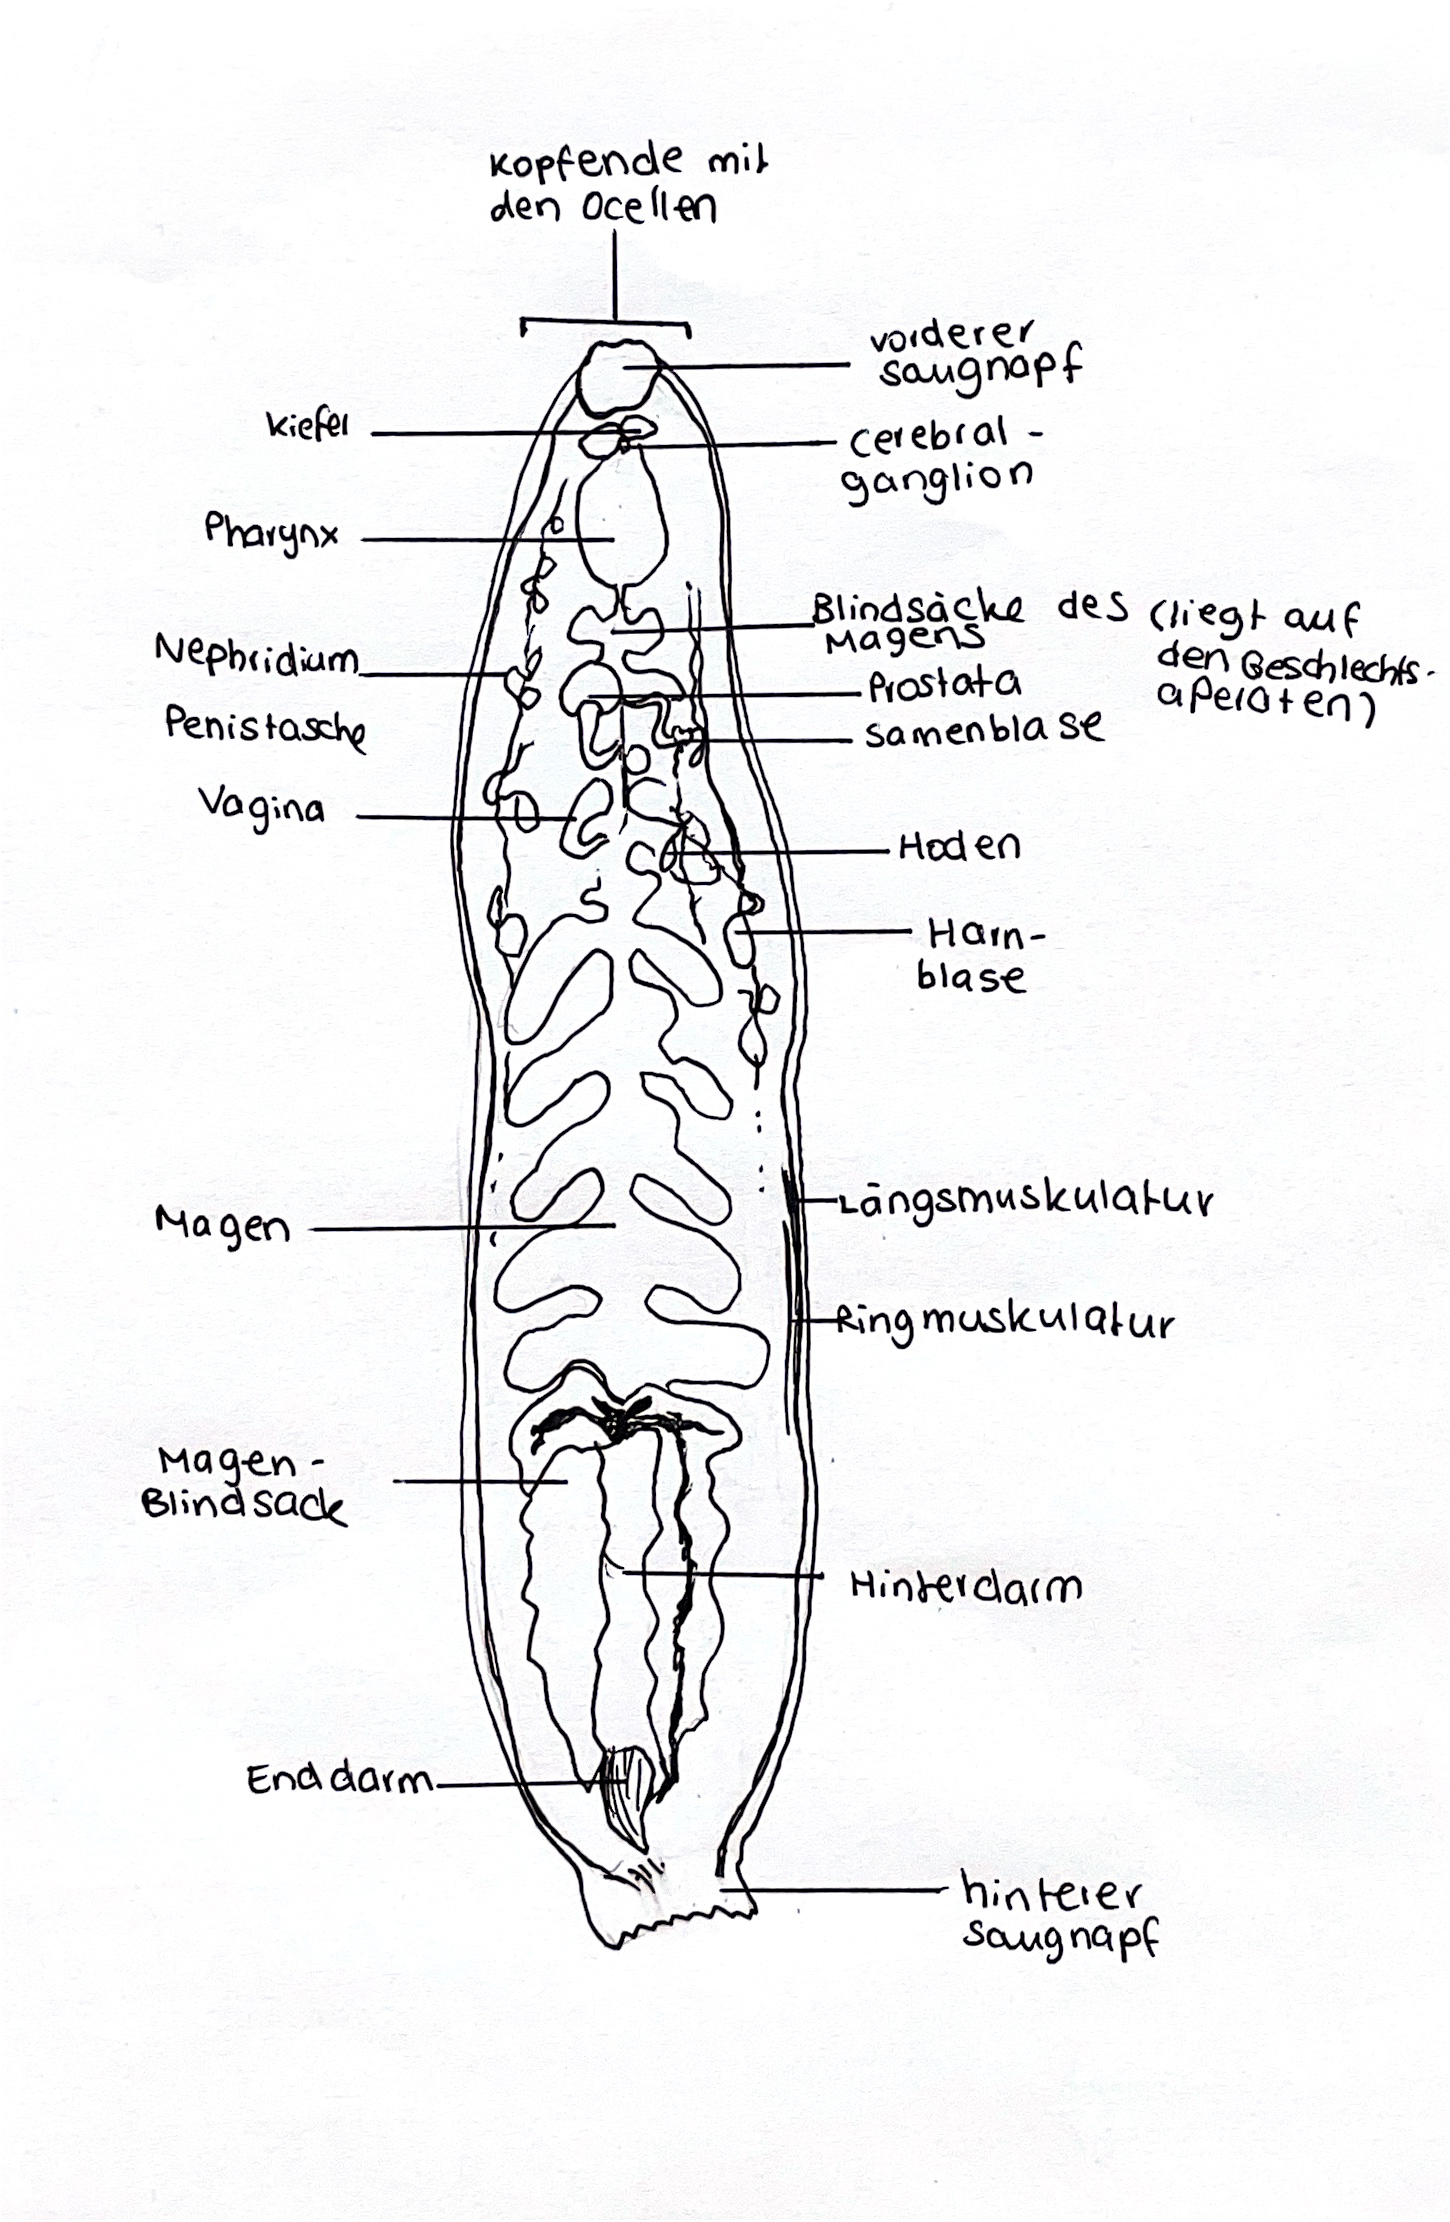
\includegraphics[scale=0.25]{Egel.JPG}
			\caption{Anatomie eines Medizinischen Egels (Hirudo verbana)}
			\label{fig:Egel_ana}
		\end{figure}
		
		\begin{figure}[H]
			\centering
			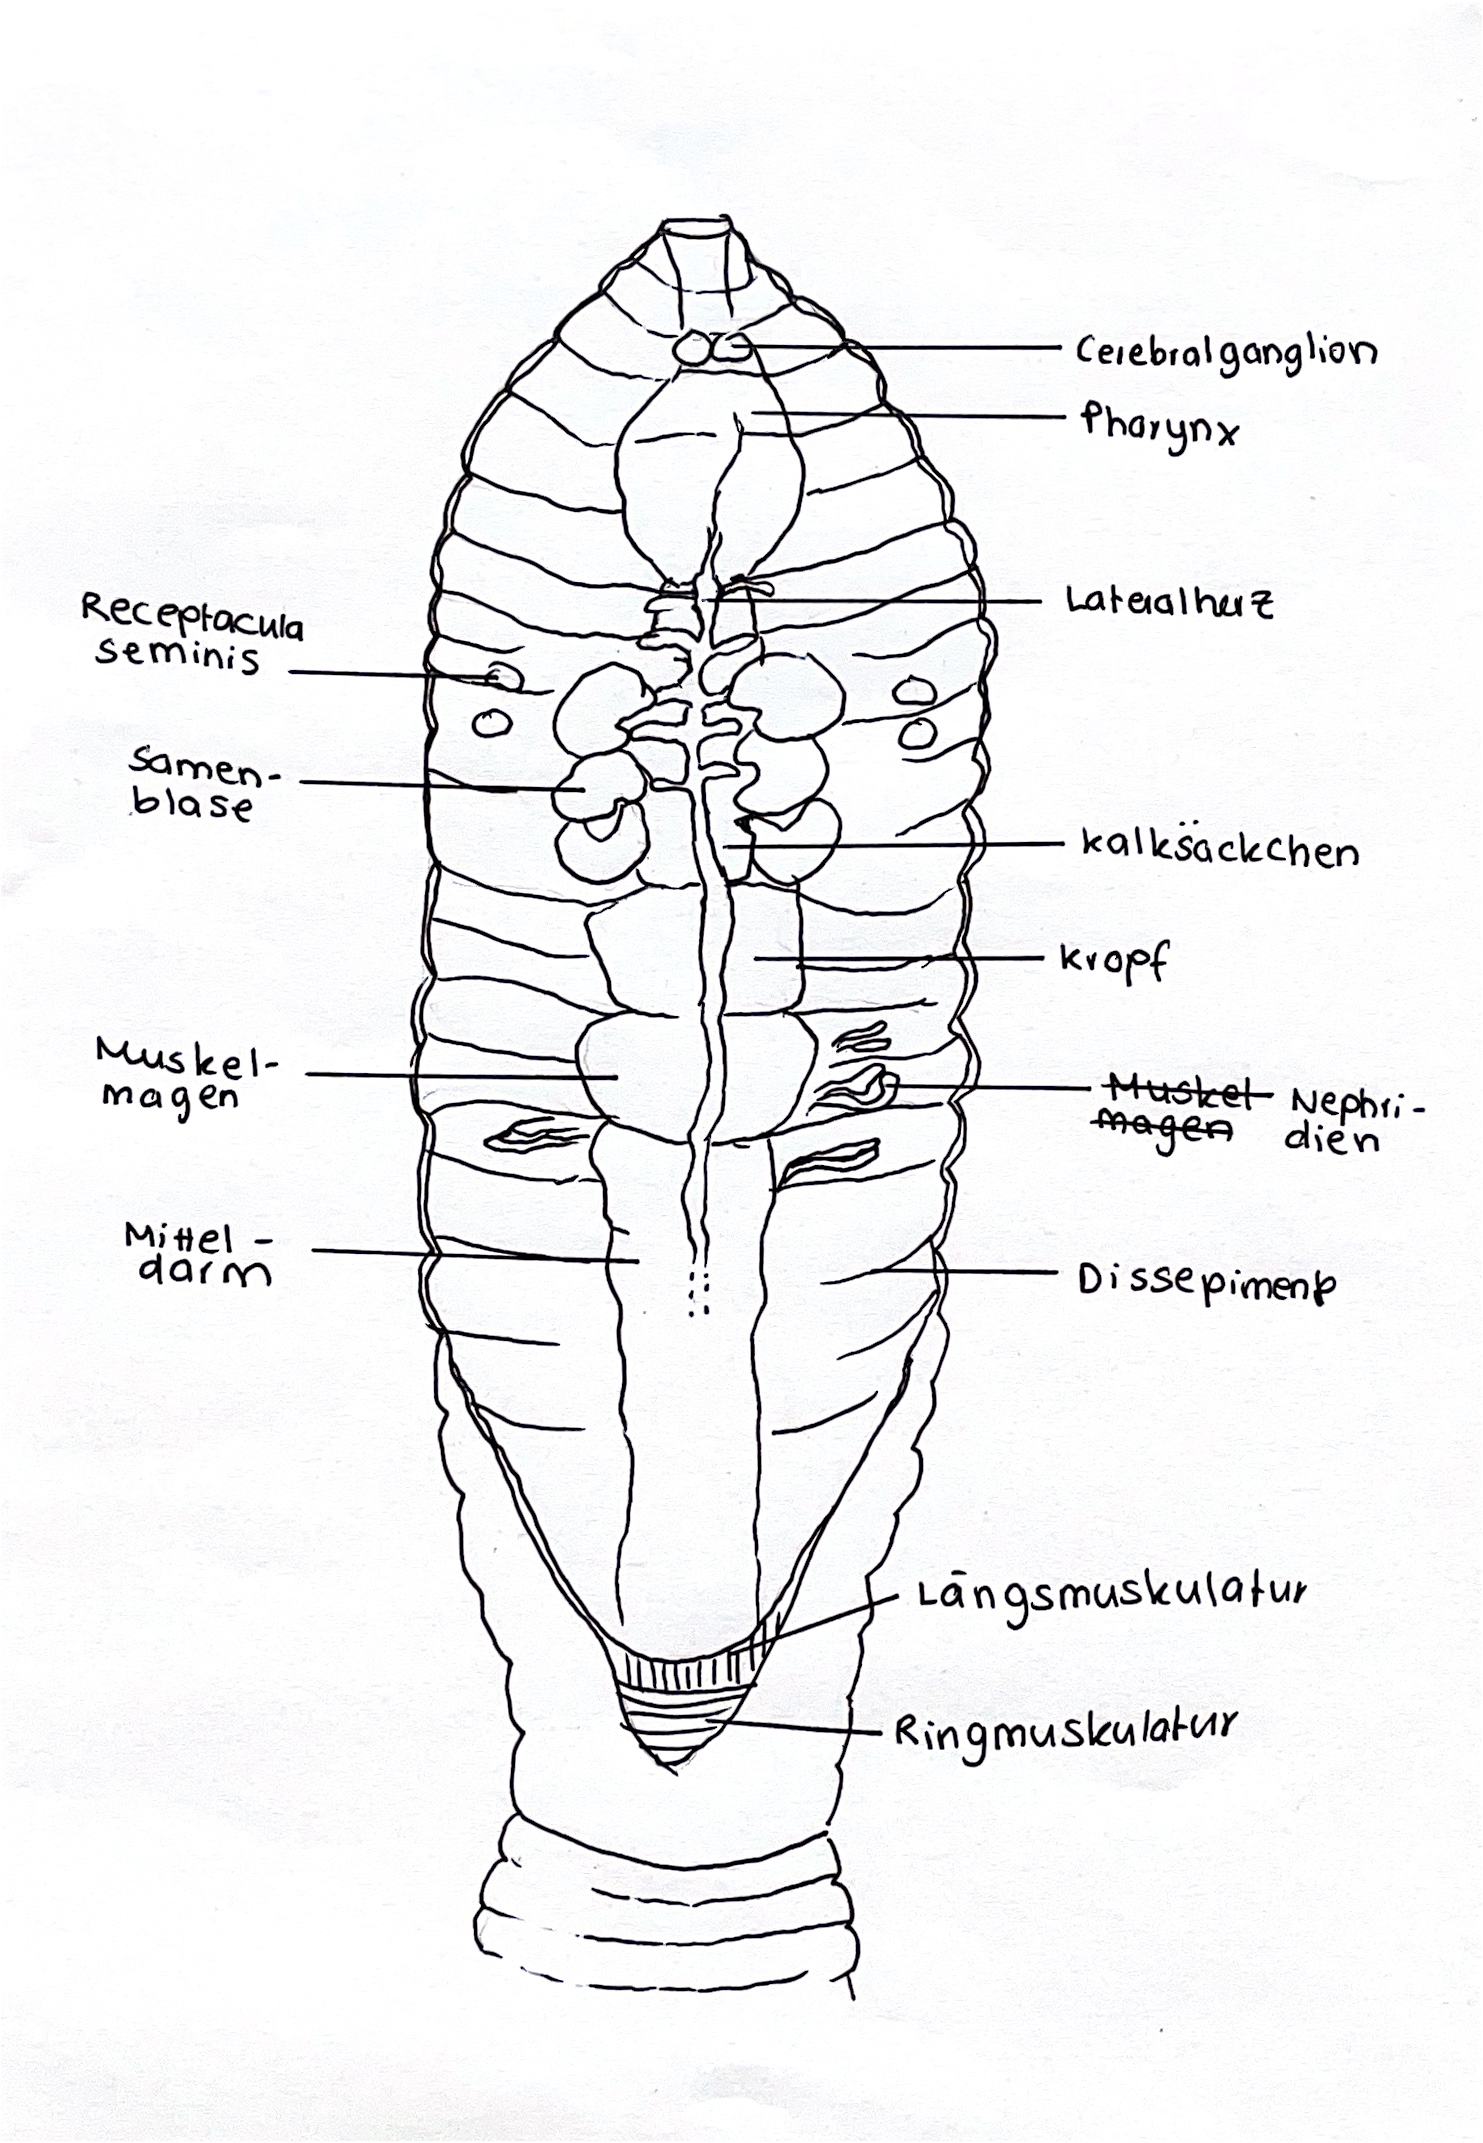
\includegraphics[scale=0.25]{Regenwurm.JPG}
			\caption{Anatomie eines Regenwurmes (Limbricus terrestris)}
			\label{fig:Regenwurm_ana}
		\end{figure}
		
		
		
		
	\addcontentsline{toc}{section}{Bibliography}
	\bibliographystyle{plainurl}
	\nocite{*}
	\bibliography{Literatur}
	\newpage
\end{document}